\section{Attack Trees}
Based on the model of the system describing the relations between actors and devices, a brainstorming session in the project group has led to a set of possible attacks on the system.
One of these attacks has been detailed in an attack tree, describing the steps an attacker would take to carry out this attack.

The attack in question is one where the consumer will attempt to have the smart meter report a lower power consumption than the actual consumption.
Doing this the user will expect a smaller bill from his electrical company.
The attack tree is presented in \cref{report_power_attack_tree}.

\begin{figure}
  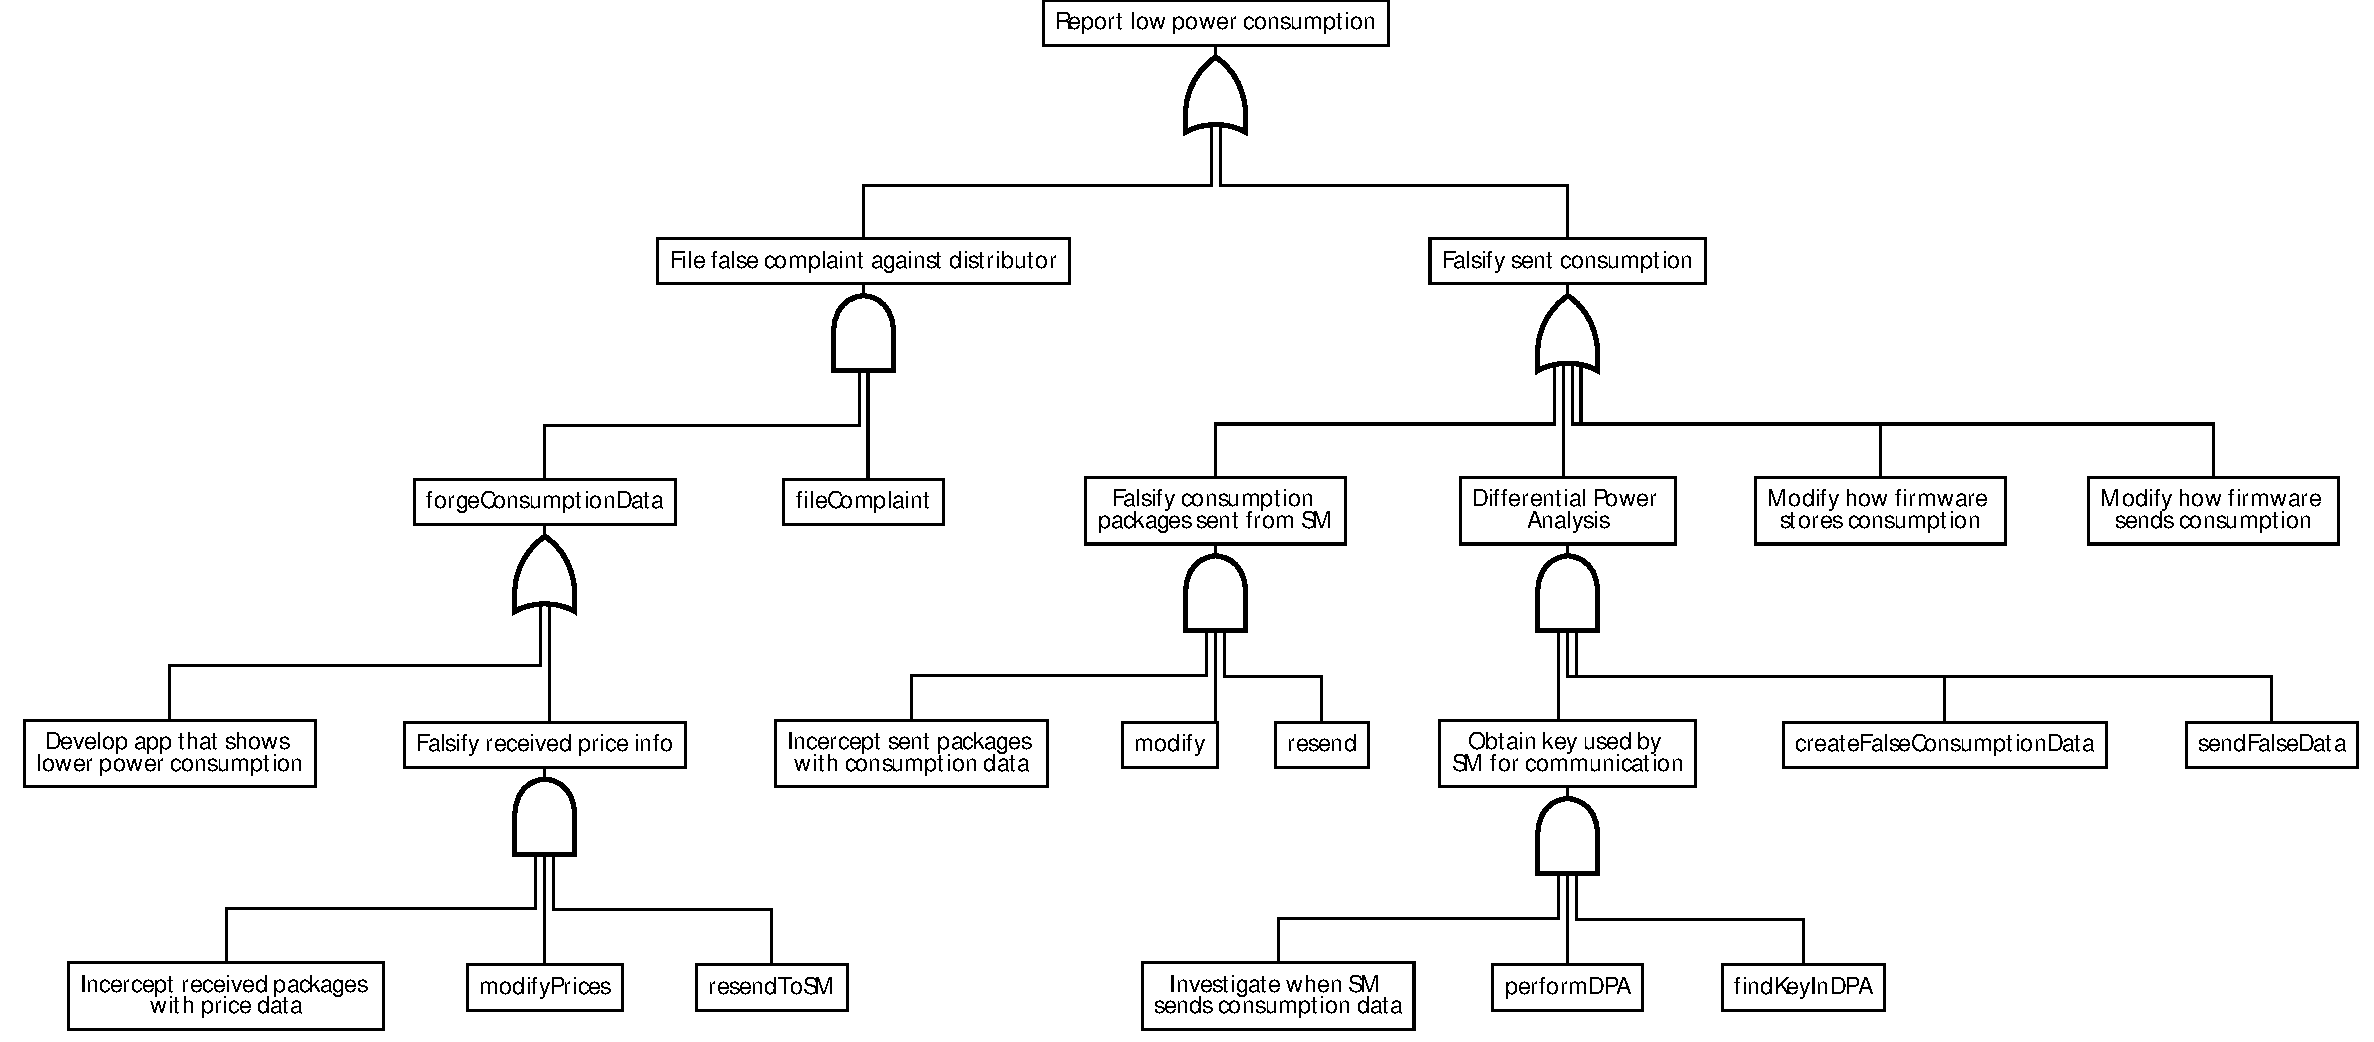
\includegraphics[width=\textheight, angle=90]{graphviz/consumer.pdf}
  \caption{An attack tree where the costumer tries to report a low power consumption.}
  \label{report_power_attack_tree}
\end{figure}

\paragraph{Definition of an attack tree}
Attack trees consist of a set of nodes representing steps in a possible attack.
The root node being the goal and leaf nodes being different ways to achieve this goal.
Inner nodes are represented as logic gates such that they do not represent a possible attack themselves but rather a rule describing how their children should be aggregated.
Thus a node represented by an AND gate would require all its child-nodes to be carried out successfully for it to be carried out successfully.

To say something about an attack tree, for instance how feasible it is, nodes can have different values corresponding to different variables(Boolean and continuous).
For instance a variable could be \textit{cost} and the values assigned to it could be in dollars.
Attack trees can show you which attacks are possible for which attackers.
For instance an attacker with a lot of money has the possibility to do all the expensive attacks where a poor attacker has not.
Also if one builds a system where the data that is getting protected is not very important, it might only be important to defend against cheap attacks.
Making attack trees takes a lot of time and effort as one has to study the security measures in place, the possible attacks and the possible attackers and outline this information in one or more attack tree(s).\cite{schneier_attack_trees}

Additionally it should be noted that the attack tree is technically not a tree as it allows for the reuse of subnodes.
This is done to illustrate how certain steps can be part of multiple attacks.
We will however continue to use the term \emph{``attack trees''} to describe these structures.
